\section{Solution}\label{sec:solution}
\subsection{Localization}\label{subsec:solution_localization}
For the localisation, a Kalman Filter (KF) or Extended Kalman Filter (EKF) \cite{b12} (according to the considered dynamic) and a distributed Weighted Least Square (WLS) have been used. In particular, each agent localises itself by running a KF/EKF that updates its prediction with only an absolute measurement (i.e. from the GPS). In the following step, each agent measures the relative distance from the others and then projects them back in the world reference frame (i.e. a frame common for all the parachutes). Finally, the network runs a distributed WLS to share the knowledge with the team in a distributed way. The KF/EKF works as an optimal filter under the hypothesis that the noise acting on the system is white, gaussian with zero mean, and uncorrelated from the one acting on the measurement, the sensors are calibrated and affected by a zero mean white noise.\\
 To reach the average consensus, the transition matrix describing the system at each time step has to be doubly stochastic, implying that the communication between agents has to be bidirectional.\\
 The distribution of the localisation has been done by applying the distributed WLS algorithm presented in the course \cite{b13}, with the Metropolis-Hastings weighting that ensures faster convergence with respect to the Maximum Degree \cite{b13}. In particular, each agent \textit{i} able to communicate with another shares its localisation and the one done on the others \textit{j} in the swarm, alongside the associated covariance matrices. The assumption on which the algorithm is based is that the localisation done by \textit{i} on the agent \textit{$j_1$} is uncorrelated to the one done on \textit{$j_2$}, which implies that the covariance matrix (called C in \cite{b13}) build during the consensus is block diagonal (even though each block is not necessarily diagonal). \\
The result of the consensus is that each agent may have improved the localisation on others that have already seen, but also for some further that were not directly measured before, and for which the information comes with message exchange. Note that now, the self-localisation of agent \textit{i} depends also on the self-localisation of the others (which is embedded in the relative measurement). This implies that agent \textit{i} cannot use the consensus output as input of the new round of KF/EKF because KFs/EKFs cannot be used in cascade. For this reason, before running another round of localisation, each agent discards the information of its position reached with the WLS. Hence, the \textit{previous} at KF/EKF step k+1 is the output of step k. This is done to ensure that the input of a KF is uncorrelated from the output of the others.\\
The picture considers the probability of performing the GPS and the relative distance measurement.
\subsection{Collision avoidance}
After localising each agent, collision avoidance is necessary to let each robot be reasonably further from the others to avoid getting tangled when moving in space. This requirement must also be fulfilled while the agents are moving in a 3D environment, considering the parachute's finite size and the knowledge of the position of only a subset of agents (with a certain level of uncertainty). All these features may be well obtained by dividing the working space with a Voronoi tessellation and enforcing each agent to move remaining inside its cell. \\
The basic idea behind the tessellation is to assign to an agent \textit{i} all the points of the mission space $q \in \mathcal{Q} \subseteq \mathbb{R}^2$ closer to it more than to the others agents \textit{j} \cite{b1}:
\begin{equation}
    \mathcal{V}_i = \left\{ q \in \mathcal{Q} \lvert \left\lVert q-p_i \right\rVert \leq \left\lVert q-\hat{p_j} \right\rVert, \forall j \neq i, j \in \tilde{\mathcal{N}_{i}} \right\}
\end{equation}
where $p_i=\left[x_i, y_i\right]^T$ is the location of the agent \textit{i} while $\hat{p_j}$ is the one of agent \textit{j} (eventually properly projected to achieve some further features, as will be explained in \autoref{sec:implementation_details}).\\
The decentralisation of the algorithm implies that each agent performs the tessellation of only a surrounding area of radius $R_s$, called \textit{sensing range}, which is usually set at $R_s = R_c/2$, with $R_c$ the furthest distance from where an agent can measure the position of another, called \textit{communication range}. The \textit{neighbour set} $\tilde{\mathcal{N}_{i}}$ is composed of all the agents for which the position is known either by consensus or direct measure. \\
During the navigation, the entity used to represent the agent is its centroid. Hence, all the computations are done to ensure that this specific point remains inside the designed area. The finite dimension of the agent $\delta_i$ has to be taken into account because otherwise, the parachute may exceed the prescribed limit even though its centroid remains inside the cell. To avoid this, the dimension of the tessellation has to be shrunk such that when the centre of the agent reaches the new edge, its encumbrance arrives at the old limit. Furthermore, since the algorithm is implemented in discrete time, the system's evolution between one instant and the following has to be considered beforehand, assuming that the agent may always move of the maximum amount allowed by the actuators in one time step.\\
Given that the environment where the parachutes fly is a 3D space, the Voronoi tessellation must be expanded at the whole volume of movement. However, the problem can still be seen as a planar one by projecting the location of the surrounding agents in the plane of the one doing the tessellation when these are reasonably close to each other. Furthermore, if the chute admits an actuation in the vertical direction, then the tessellation concept can be extended in the vertical axis to ensure collision avoidance even in that dimension. The safe space is between the agents and a minimum height called $z_{min}$.

\subsection{High-level motion control}
The high-level motion control deals with the problem of how and where to move the centroid to make it land on the target. Furthermore, since the centroid is a function of the single parachute location, it coordinates the agents' movements to realise the prescribed centroid trajectory. Instead, the actuators commands enabling this displacement are synthesised by the \textit{low-level controller}.\\
In this work, the centroid is modelled as a fictional fully actuated parachute with a linear dynamic in 2 dimensions, as shown in (\ref{robot}), while the gravity ensures the convergence in the z-direction.
\begin{equation}
    \begin{bmatrix}
        x_{i+1}\\
        y_{i+1}
    \end{bmatrix}=
    \begin{bmatrix}
        I_2
    \end{bmatrix}
    \begin{bmatrix}
        x_i\\
        y_i
    \end{bmatrix}
    +\Delta t\begin{bmatrix}
        I_2
    \end{bmatrix}
    \begin{bmatrix}
        v_{x,i}\\
        v_{y,i}
    \end{bmatrix}
    \label{robot}
\end{equation}
An LQR algorithm \cite{b15} has been used to find the optimal input $u$ to be fed to the fake agent. This algorithm can only be used for linear systems, and it finds the global optimum of the problem, which is calculated by means of a minimisation of a cost function, expressed as:
\begin{equation}
    J = \sum_{k=t}^{N-1} x_k^TSx_k + u_k^TRu_k
\end{equation}
where $S$ and $R$ are the state and input cost matrices, which can be modelled to improve the state or the input minimisation, and $x$ and $u$ are the actual state and input.\\
In the discrete time, finite horizon domain, the optimum input is given by:
\begin{equation}
    u_t=K_tx_t 
\end{equation}
where $K_t$ is the optimal gain matrix given by the algorithm.\\
Once the optimal control for the fictional robot is found, following the kinematics shown in the equations (\ref{robot}), its next desired position is calculated.\\
The computation of each parachute's desired position that realises the global centroid's desired movement is not trivial. The global centroid is a function of each parachute position, and the inverse kinematic (i.e. finding the parachutes' positions that realise a desired position of the centroid) is over-determined. Two solutions have been proposed to solve this problem. At the same time, a third one to be used in some \textit{emergency} situations to avoid collision will be presented in \autoref{sec:details_high_level} after the reasons why it is necessary.
\subsubsection{Same control for all the chutes}
 A quick and intuitive but "forced" solution consists of feeding the same control input in the parachutes found in the LQR problem since if every parachute moves similarly, the global centroid will be moved accordingly.
 \subsubsection{Inverse kinematics}
  A more robust solution comes from comparing this problem to the well-known and solved problem of redundancy in robotics. In fact, as in over-actuated manipulators, infinite joints' configurations realise a desired end effector position; here, infinite agents' locations realise the centroid one. However, a numerical approach has been developed in the past years to solve inverse kinematics by a \textit{postural task}, which is just an arbitrarily chosen secondary task in the joint space that does not affect the motion of the end-effector  but identifies one solution among the infinite ones \cite{b5} \cite{b6}.\\
In this specific case, two possible secondary tasks may be to let every single agent converge toward the land target or the global centroid. The algorithm can prioritise principal or secondary requirements according to a weighting value that can be chosen arbitrarily.

\subsection{Low-level motion control}
Given the single parachute target point from the high-level control, the goal of the low-level control is to provide the input that ensures the move towards it while not exceeding the motion boundaries identified by the Voronoi tessellation. 
\subsubsection{Control of linear model}
In the case of linear dynamics, one possible control law is the one proposed by \cite{b1}:
\begin{gather}
    \label{eq:proportional}
    u=-k_p\left(p_i - C_{\mathcal{V}_i}\right)\\
    \label{centroid}
    C_{\mathcal{V}_i} = \frac{1}{M_{\mathcal{V}_i}}\int_{\mathcal{V}_i}\varphi\left(q\right)qdq \text{ , } M_{\mathcal{V}_i} = \int_{\mathcal{V}_i}\varphi\left(q\right)dq
\end{gather}
with, for the planar motion, $\varphi\left(q\right)$ is a bivariate pdf centred in the point identified by the high-level control. This law uses the property that each point inside the Voronoi cell can be reached by the agent with a straight motion.\\
Regarding the control on the vertical axis, as said before, the velocity input has to be constrained. In particular, a proportional gain has been chosen to break when the $z_{min}$ is near the parachute:
\begin{equation}
\label{control_law_z}
    \begin{gathered}
        k_{pz}=-\bar{v}_z/R_{sv}\\
        u_{tmp}=-\bar{v}_z-k_{pz}(z_i-z_{min,i})\\
        v_z=\min(u_{tmp}, v_{z,min}-\bar{v}_z)
    \end{gathered}
\end{equation}
In this way, when there are no parachutes under the agent $i$, $(z_i-z_{min,i})=R_{sv}$ and so the control $v_z$ is zero, meaning that there is no need to break. On the other hand, when $(z_i-z_{min,i})=0$, meaning that the parachute would not want to go down because the other agents are too near, the input is $v_{z,min}-\bar{v}_z$, such that when in the dynamics it is added the effect of gravity (\ref{eq:model_1},\ref{eq:NL}) the sum results in the minimum vertical velocity: the agent cannot stop in the air but has to descent with some velocity.\\
Since the external disturbances act directly on the positions, the effective velocities can be locally greater or smaller than the boundaries.
\subsubsection{Control of the unicycle model}
Since the trajectory followed by the non-linear agents may exceed the Voronoi cell limits if (\ref{control_law_z}) is employed, a more complex one must be used. In this work, the control law (\ref{eq:control_law}) \cite{b4} allows to guarantee the convergence of the parachute towards the target in a fast and elegant way (without the use of a PID controller), and also to find the so-called \textit{Feedback Motion Predict (FMP)}, which is the area that the parachute can occupy during the execution of the control law (\ref{eq:control_law}).
\begin{equation}
\label{eq:control_law}
    \begin{gathered}
        v_y = k_v\max\Big(0,\begin{bmatrix}
           \cos{\theta} & \sin{\theta}
       \end{bmatrix}(C_{\mathcal{V}_i} -p_i)\Big)\\
        \omega = k_{\omega}\atantwo\Big(\begin{bmatrix}
           -\sin{\theta} \\ \cos{\theta}
       \end{bmatrix}^T(C_{\mathcal{V}_i} -p_i),\begin{bmatrix}
           \cos{\theta} \\ \sin{\theta}
       \end{bmatrix}^T(C_{\mathcal{V}_i} -p_i)\Big)
    \end{gathered}
\end{equation}
\begin{figure}[h]
    \centering
    \subfloat[][\emph{Truncated Ice-Cream Motion Cone updating as the agent moves.}]{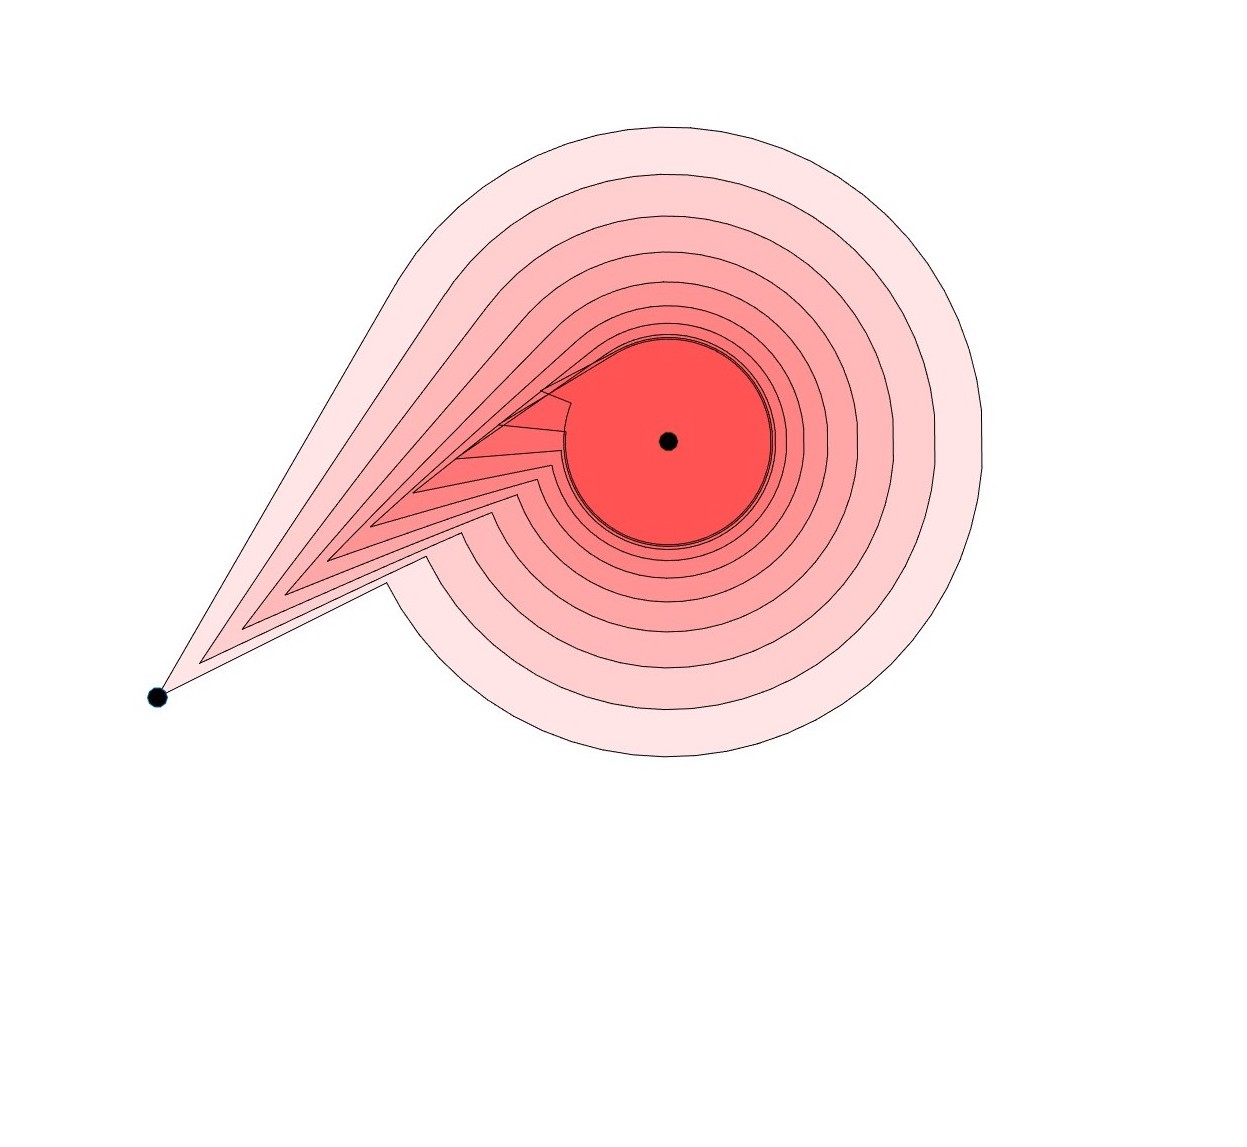
\includegraphics[scale=.08]{images/cone.jpg}} \quad
    \subfloat[][\emph{The cone is moved to be fit into the Voronoi cell.}]{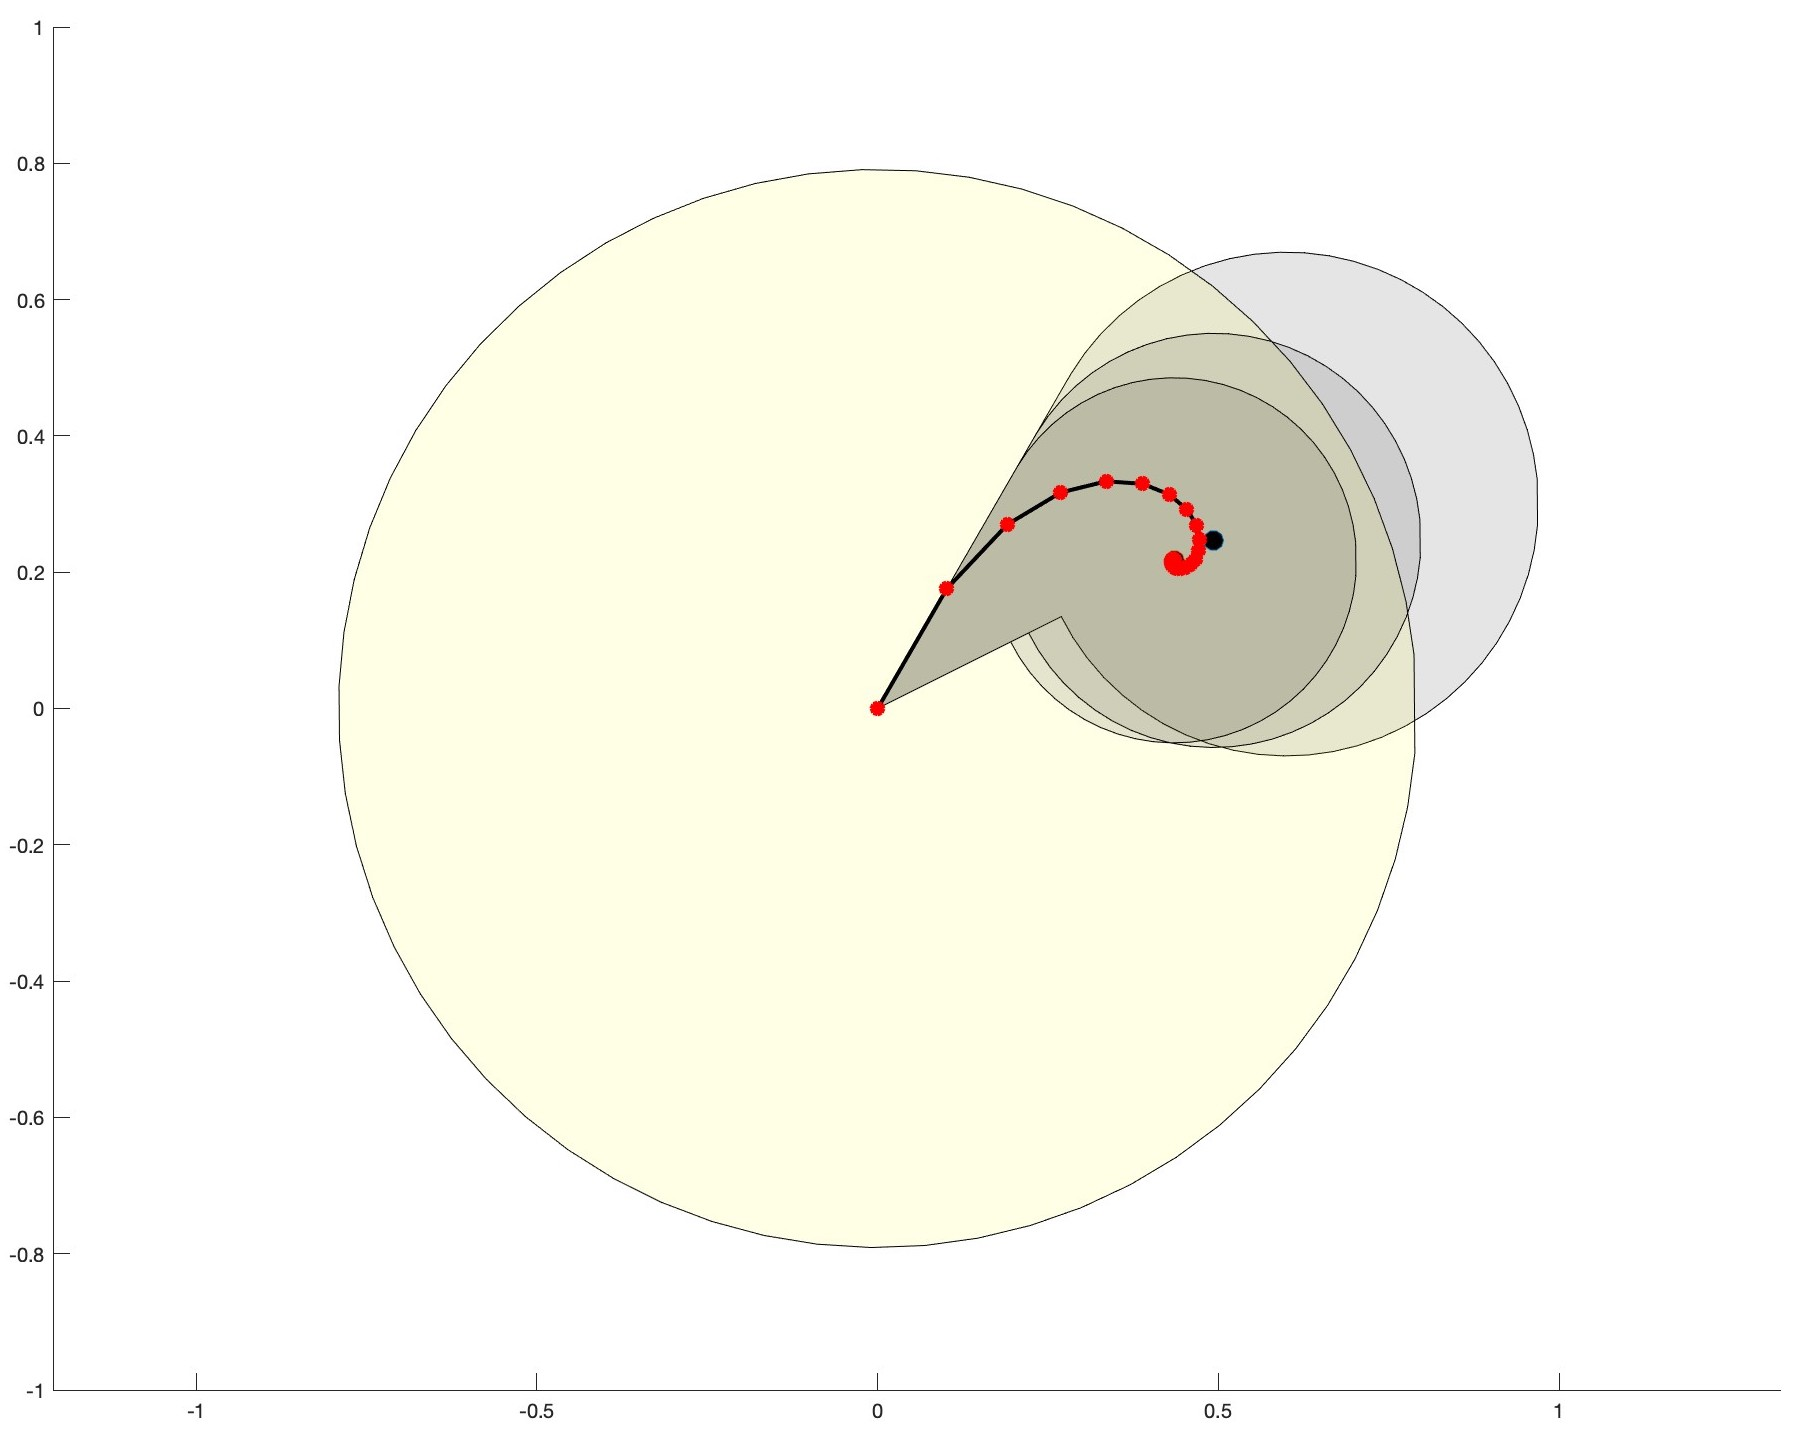
\includegraphics[scale=.07]{images/mot_pred.jpg}}
    \caption{Feedback Motion Prediction area for non-linear dynamics.}
    \label{fig:motion_pred}
\end{figure}

As mentioned in section \ref{unicyle}, the forward velocity is saturated to zero, so the parachute can never move backwards. Furthermore, it is not forced to move at a minimum velocity, as in the real chutes. This assumption simplifies the control because, in the case of non-zero positive minimum velocity (and at least with this control policy), there is no guarantee that the parachute will not exit the Voronoi cell, for example, when it is too close to the boundary.\\
To make sure that the parachute will not violate the Voronoi cell boundary, the FMP is initially calculated and if it exits the cell, the arrival point (i.e. the new centroid founded by (\ref{centroid})) is moved closer to the actual position of parachute iteratively until the FMP fits into the Voronoi cell (as could be seen in \autoref{fig:motion_pred}b). \cite{b4} proposed different ways to define valid FMP, and among them, it is chosen the \textit{Truncated Ice-Cream Motion Cone} because it is the least conservative but smaller one (Figure \ref{fig:motion_pred}a).